\documentclass[11pt, a4paper]{article}
%\usepackage{proj1}
\usepackage{natbib}
\usepackage{fancyhdr}  
\usepackage{subcaption}
\usepackage{caption}
\usepackage{graphicx}
\usepackage{numprint}
\usepackage{multirow}
\linespread{1.25} 
\setlength{\parindent}{0cm}
\graphicspath{{Images/}}
\usepackage{hyperref}
\usepackage{amsmath}
\usepackage{amsfonts}
\usepackage{amssymb}
\usepackage{amsthm}
\usepackage{mathtools}
\usepackage{commath}
\usepackage{bbm}

%\usepackage[sc,osf]{mathpazo}
\usepackage{subcaption}
\usepackage[a4paper, top=1in, left=1.0in, right=1.0in, bottom=1in, includehead, includefoot]{geometry} %Usually have top as 1in

\usepackage{listings}
\usepackage{color} %red, green, blue, yellow, cyan, magenta, black, white
\definecolor{mygreen}{RGB}{28,172,0} % color values Red, Green, Blue
\definecolor{mylilas}{RGB}{170,55,241}


\hypersetup{colorlinks,linkcolor={black},citecolor={blue},urlcolor={black}}
\usepackage{color}
\urlstyle{same}


\theoremstyle{definition}
\newtheorem{definition}{Definition}[section]

\newcommand{\adja}{q_a}
\newcommand{\adjb}{q_b}
\newcommand{\adjaB}{q_{a,\partial \Omega}}
\newcommand{\adjbB}{q_{b,\partial \Omega}}
\newcommand{\adjB}{q_{\partial \Omega}}
\newcommand{\Adja}{\mathbf{p}}
\newcommand{\Adjb}{q}
\newcommand{\adj}{q}
\newcommand{\Adjc}{{q}_{\partial \Omega}}
\newcommand{\ra}{\rho_a}
\newcommand{\rb}{\rho_b}
\newcommand{\w}{\mathbf{w}}
\newcommand{\f}{\mathbf{f}}
\newcommand{\ve}{\mathbf{v}}
\newcommand{\n}{\mathbf{n}}
\newcommand{\h}{\mathbf{h}}
\newcommand{\K}{\mathbf{K}}
\newcommand{\hr}{\widehat \rho}

%	\begin{figure}[h]
%		\centering
%		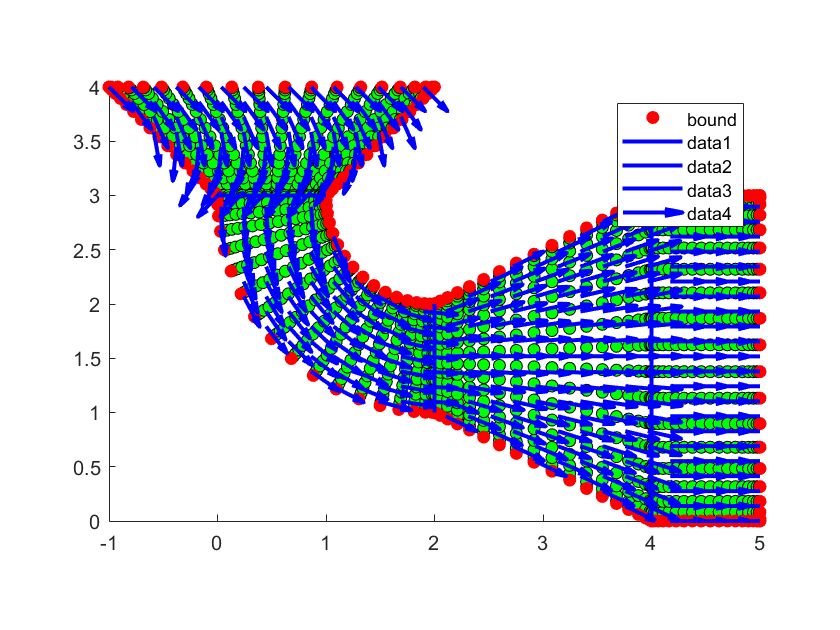
\includegraphics[scale=0.35]{F1.png}
%		\caption{Forward $\rho$ for $a = 0.01$} 
%		\label{F1}
%	\end{figure}

\begin{document}


	
	\section{Periodic Boundary Conditions}
	We consider the advection diffusion equation with periodic boundary conditions and a corresponding OCP:
	\begin{align*}
		&\min \frac{1}{2}|| \rho - \hr||^2 + \frac{\beta}{2}||\w||^2\\
		&\text{subject to:}\\
		&\frac{\partial \rho}{\partial t} = \frac{\partial^2 \rho}{\partial x^2} - \frac{\partial \rho \w}{\partial x}\\
		& \rho(a) = \rho(b)\\
		& \frac{\partial \rho(a)}{\partial x} - \rho(a) \w(a) = -\frac{\partial \rho(b)}{\partial x}  + \rho(b) \w(b)
	\end{align*}
	The relevant part of the Lagrangian is then:
	\begin{align*}
		\mathcal{L} &= ... -\int_0^T \int_\Omega \left(\frac{\partial \rho}{\partial t} - \frac{\partial^2 \rho}{\partial x^2} + \frac{\partial \rho \w}{\partial x}\right)q dr dt \\
		&- \int_0^T \left(\rho(b)q_1 - \rho(a)q_1 + \frac{\partial \rho(b)}{\partial x}q_2 - \rho(b)\w(b)q_2 + \frac{\partial \rho(a)}{\partial x}q_2 - \rho(a)\w(a)q_2\right) dt.
	\end{align*}
	Taking partial derivatives, the relevant part of the Lagrangian is:
	\begin{align*}
		\mathcal{L} = ... - \int_0^T \left[q \frac{\partial \rho}{\partial x} - \rho\frac{\partial q}{\partial x} - \rho \w q\right]_a^b -
		\left(\rho(b)q_1 - \rho(a)q_1 + \frac{\partial \rho(b)}{\partial x}q_2 - \rho(b)\w(b)q_2 + \frac{\partial \rho(a)}{\partial x}q_2 - \rho(a)\w(a)q_2\right)dt.
	\end{align*}
	Taking the derivative with respect to $\rho$ gives:
	\begin{align*}
		\mathcal{L}_\rho h &= ... - \int_0^T \left[q \frac{\partial h}{\partial x} - h\frac{\partial q}{\partial x} - h \w q\right]_a^b \\
		&-
		\left(h(b)q_1 - h(a)q_1 + \frac{\partial h(b)}{\partial x}q_2 - h(b)\w(b)q_2 + \frac{\partial h(a)}{\partial x}q_2 - h(a)\w(a)q_2\right)dt
	\end{align*}
	Writing all terms explicitly:
	\begin{align*}
		\mathcal{L}_\rho h &= ... + \int_0^T \bigg(- q(b) \frac{\partial h(b)}{\partial x} + h(b)\frac{\partial q}{\partial x} + h(b) \w(b) q(b) + q(a) \frac{\partial h (a)}{\partial x} - h(a)\frac{\partial q(a)}{\partial x} - h(a) \w(a) q(a)  \\
		&- h(b)q_1 + h(a)q_1 - \frac{\partial h(b)}{\partial x} q_2 + h(b)\w(b)q_2 - \frac{\partial h(a)}{\partial x}q_2 + h(a)\w(a)q_2 \bigg)dt
	\end{align*}
	Then considering the terms that satisfy $\frac{\partial h}{\partial x} \neq 0$ we get:
	\begin{align*}
		- q(b) + q(a) -q_2(b) - q_2(a) =0,
	\end{align*}
	so that $q(b) = -q_2(b)$ and $q(a) = q_2(a)$.
 	For $h \neq 0$ we have:
	\begin{align*}
		\frac{\partial q(b)}{\partial x} + \w(b) q(b) - \frac{\partial q(a)}{\partial x} - \w(a) q(a) - q_1(b) + q_1(a) + \w(b) q_2(b) + \w(a) q_2(a) = 0 
	\end{align*}
	Using the first condition, we get:
	\begin{align*}
		\frac{\partial q(b)}{\partial x} + \w(b) q(b) - \frac{\partial q(a)}{\partial x} - \w(a) q(a) - q_1(b) + q_1(a) - \w(b) q(b) + \w(a) q(a) = 0,
	\end{align*}
	so that terms involving $\w$ cancel to give:
	\begin{align*}
		\frac{\partial q(b)}{\partial x} - \frac{\partial q(a)}{\partial x} - q_1(b) + q_1(a) = 0.
	\end{align*}
	If $q_1 = q_2$ we get:
	\begin{align*}
		\frac{\partial q(b)}{\partial x} - \frac{\partial q(a)}{\partial x} + q(b) + q(a) = 0.
	\end{align*}

\section{Time independent control}
We wanted to see whether the time independent flow control is similar to the $\nabla V_{ext}$ of the target.
The target state was influenced by $V_{ext} = 0.1 y_2$. The forward state for the OCP was influenced by $V_{ext} = 0.01 y_2$. 
Figure \ref{F1} shows the control and $\nabla V_{ext}$ of the target. Why is one positive and one negative? Is it because they are opposite signs in PDE?

	\begin{figure}[h]
		\centering
		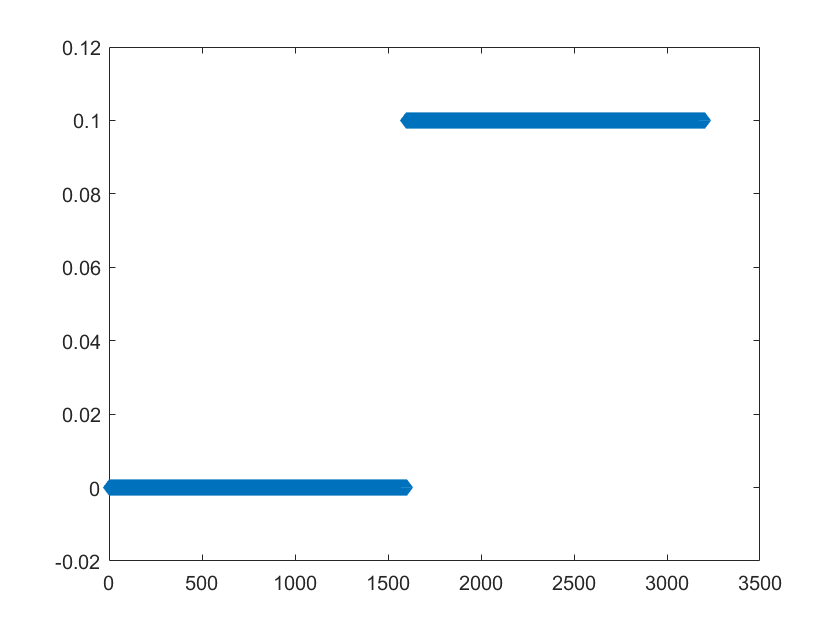
\includegraphics[scale=0.35]{V1.png}
		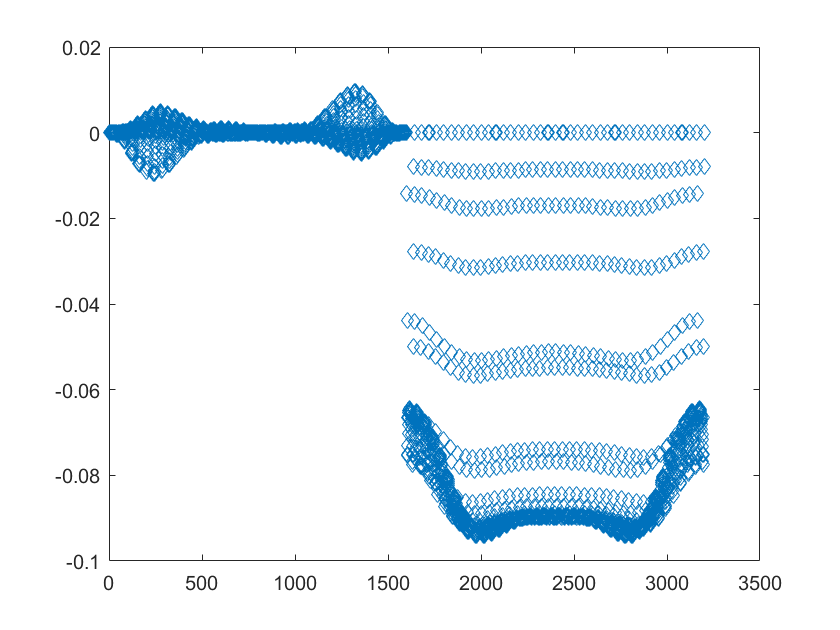
\includegraphics[scale=0.35]{W1.png}
		\caption{$\nabla V_{ext}$ of target and optimal control} 
		\label{F1}
	\end{figure}

\section{Multishape Channel}
The target flow profile works now and can be seen in Figure \ref{F2}. We chose $N = 20$, $n = 20$ for each shape and $T = 5$. 
The optimal control problem is still not quite working. For $\beta = 10^{-1}$, it seems to work or almost, but for $10^{-3}$ it converges in three iterations, where the last error is zero. However, $J_{FW} < J_{Opt}$. When decreasing $\lambda$ from $0.01$ to $0.001$, the convergence steps are smaller and hopefully therefore it will converge to a minimum. The target and optimal $\rho$ for $\beta = 10^{-1}$ are displayed in Figure \ref{F3}. We have $J_{FW} = 0.2092$ and $J_{Opt} = 0.1563$.
\begin{figure}[h]
	\centering
	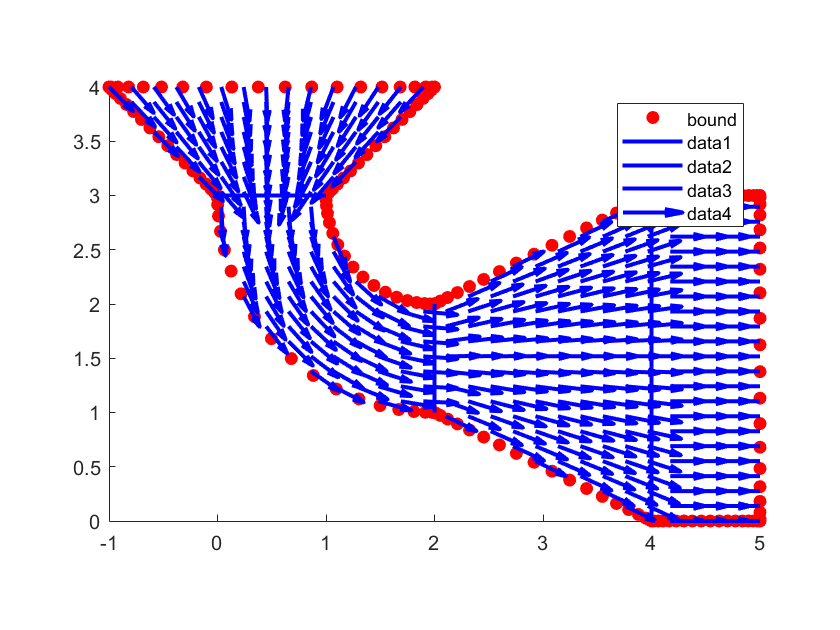
\includegraphics[scale=0.35]{S1.png}
	\caption{Target flow setup} 
	\label{F2}
\end{figure}
\begin{figure}[h]
	\centering
	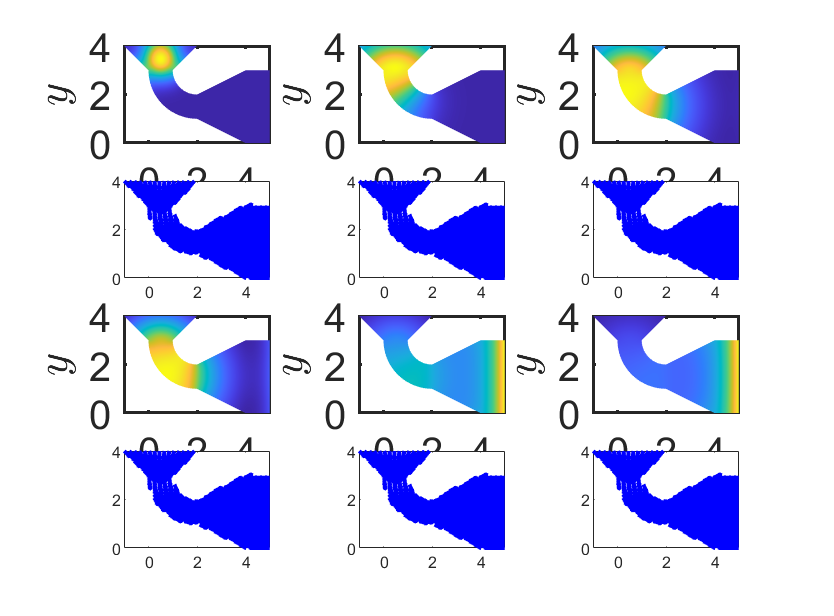
\includegraphics[scale=0.6]{R1.png}
	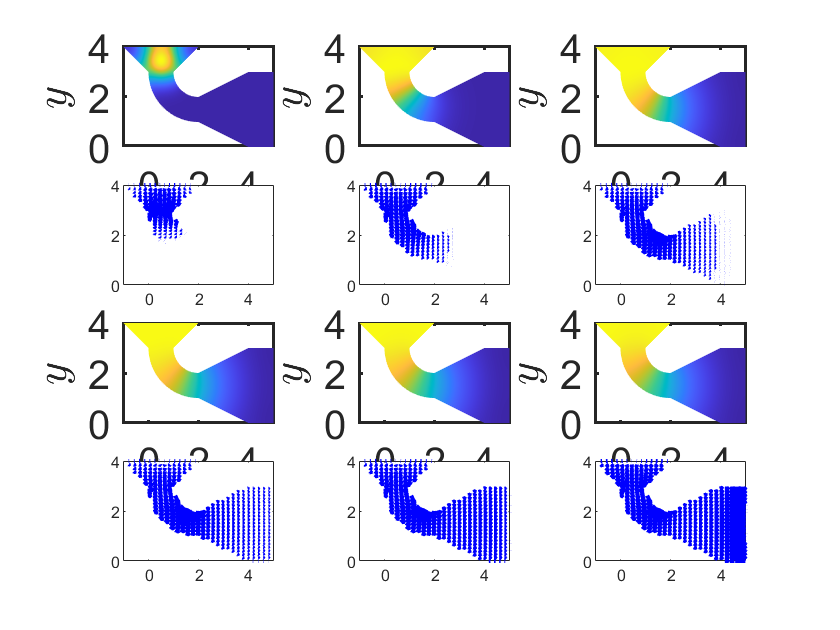
\includegraphics[scale=0.6]{R2.png}
	\caption{$\hr$ and optimal $\rho$, $\beta = 10^{-1}$.} 
	\label{F3}
\end{figure}

	- exact problem not exact yet
- multishape JFW < JOpt

\end{document}